\documentclass{article}
\usepackage{graphicx}
\graphicspath{{images/}}
\usepackage{layout}
\usepackage[a4paper, total={6in, 9in}]{geometry}
\usepackage[colorlinks = true,
            linkcolor = blue,
            urlcolor  = blue,
            citecolor = blue,
            anchorcolor = blue]{hyperref}%hiperenllaços
\usepackage[catalan]{babel}
\usepackage{minted} %Para el entorno de código
\usepackage[table,xcdraw]{xcolor}  %Para el color del entorno del código
\usepackage{enumitem}
\usepackage[T1]{fontenc}
\usepackage{setspace}
\usepackage{amsmath}
\usepackage{lipsum}
\usepackage{subfig}
\usepackage{hyperref}
\usemintedstyle{monokai}

\newcommand\myfontsize{\fontsize{13pt}{16pt}\selectfont}




\begin{document}

%TITOL
\begin{titlepage}
    \centering
    \includegraphics[width=0.75\textwidth]{images/uib.png}\par\vspace{1cm}
    {\scshape\LARGE Grado de Ingenieria Informatica \par}
    \vspace{1cm}
%Clasificación de la práctica
    {\Large Tecnologias Multimedia \par}
    \vspace{1.5cm}
%Titulo de la practica
    {\huge\bfseries Documentación Puertos Mallorca\par}
    \vspace{2cm}
%Autores / autor.
    {\large
    Jaume Adrover Fernández \\
    jaume.adrover3@estudiant.uib.cat \\
    \vspace{0.5cm}
    Marc Cañellas Gomez \\
    marc.canellas@estudiant.uib.cat \\
    \vspace{0.5cm}
    Diego Bermejo Cabañas \\
    diego.bermejo@estudiant.uib.cat \\
    \vspace{0.5cm}
    \textit{}\\
    \texttt{}
    \par}
    \vfill

% Bottom of the page
    {\large \texttt{} \\\today\par}
\end{titlepage}

\newpage
\hypersetup{linkcolor=black}
\tableofcontents
\newpage

\section{Introducción}
En este documento se explicara el contenido de la web-app que hemos desarollado de forma que se pueda entender como se ha desarrollado. Ademas, se mostraran todas sus funcionalidades para que el usuario tenga en cuenta todo lo que puede hacer con la web-app. Por otro lado, se explicacran que herramientas se han usado para el desarrollo de esta, ademas de las libreries, APIs y extras utilizados para la composición grafica de la pagina.

\section{URL}
Primero de todo se mostrara como se puede acceder a la web-app desarrollada. En nuestro caso, hemos comprado un servicio de hosting en la pagina \href{https://www.dondominio.com/es/}{dondominio.com} gracias a los codigos proporcionado por nuestro profesor de la assignatura. En nuestro caso, hemos elegido como nombre de la url para acceder a nuestra web-app \href{http://www.puertosmallorca.com/}{puertosmallorca.com}. Hemos elegido este nombre ya que lo encontramos relativamente corto, conciso y muestra muy claramente lo que podras encontrar en nuestra web-app. principalmente lo hemos elegido siguiendo las recomendaciones que se nos especificaban en la pagina de contratación del hosting.

\section{Funcionalidades de la Web-App}
Una vez explicado como hemos contratado el servicio de hosting y podemos acceder a la web-app, medinte el link proporcionado en la sección anterior, pasaremos a explicar todas las funcionalidades que el usuario puede realizar con ella.

\subsection{Home Page}
Nada más entrar al link proporcionado, encontraremos una barra de navegación que se mantiene fija en la parte superior de la pagina. En la parte de la izquierda de esta, encontramos el logo y el nombre de la web-app y tanto el logo como el nombre, serviran para que el usuario pueda volver a la homepage des de cualquier parte de la web-app con tan solo clicar encima de una de ellas. En la parte de la derecha de la barra de navegación, encontramos 3 botones para acceder a las diferentes funcionalidades que ofrece la pagina:
\begin{itemize}
    \item \textbf{Ver Puertos}: este nos llevará más abajo de la homepage, donde podremos obtener información sobre los puertos de Mallorca registrados en la pagina.
    \item \textbf{Plan de Navegación}: con este boton, podremos acceder a la pagina que nos permitirá crear una ruta maritima segun unos imputs que le permitiremos indicar al usuario. Esta, también contendrá recomendaciones de restaurantesn playas y sitios de interés cercanos durante la ruta.
    \item \textbf{Contacto}: nos llevará a una pagina donde el usuario podrá contactar con nosotros en caso de tener cualquier problema.
\end{itemize}
\begin{figure}[ht]
    \centering
    \includegraphics[width=0.95\textwidth]{images/nvbar.png}
    \caption{Barra de navegación de la web-app}
\end{figure}
Un poco más abajo de la barra de navegación, encontramos un carousel de 3 fotos con textos encima de estas. En la primera de ellas se da la biembenida al usuario, en la segunda, se muestra que puedes encontrar información sobre los puertos de mallorca y en la terceraq que puedes crear tu plan de navegación. Con esto, damos a conocer de manera simple y concisa lo que el usuario puede hacer con nuestra web-app. El usuario se puede desplazar de forma manual por las fotos del carousel, y también existe una flecha que apunta hacia abajo que nos llevará a la siguiente sección de la homepage.
\newpage
\begin{figure}[ht]
    \centering
    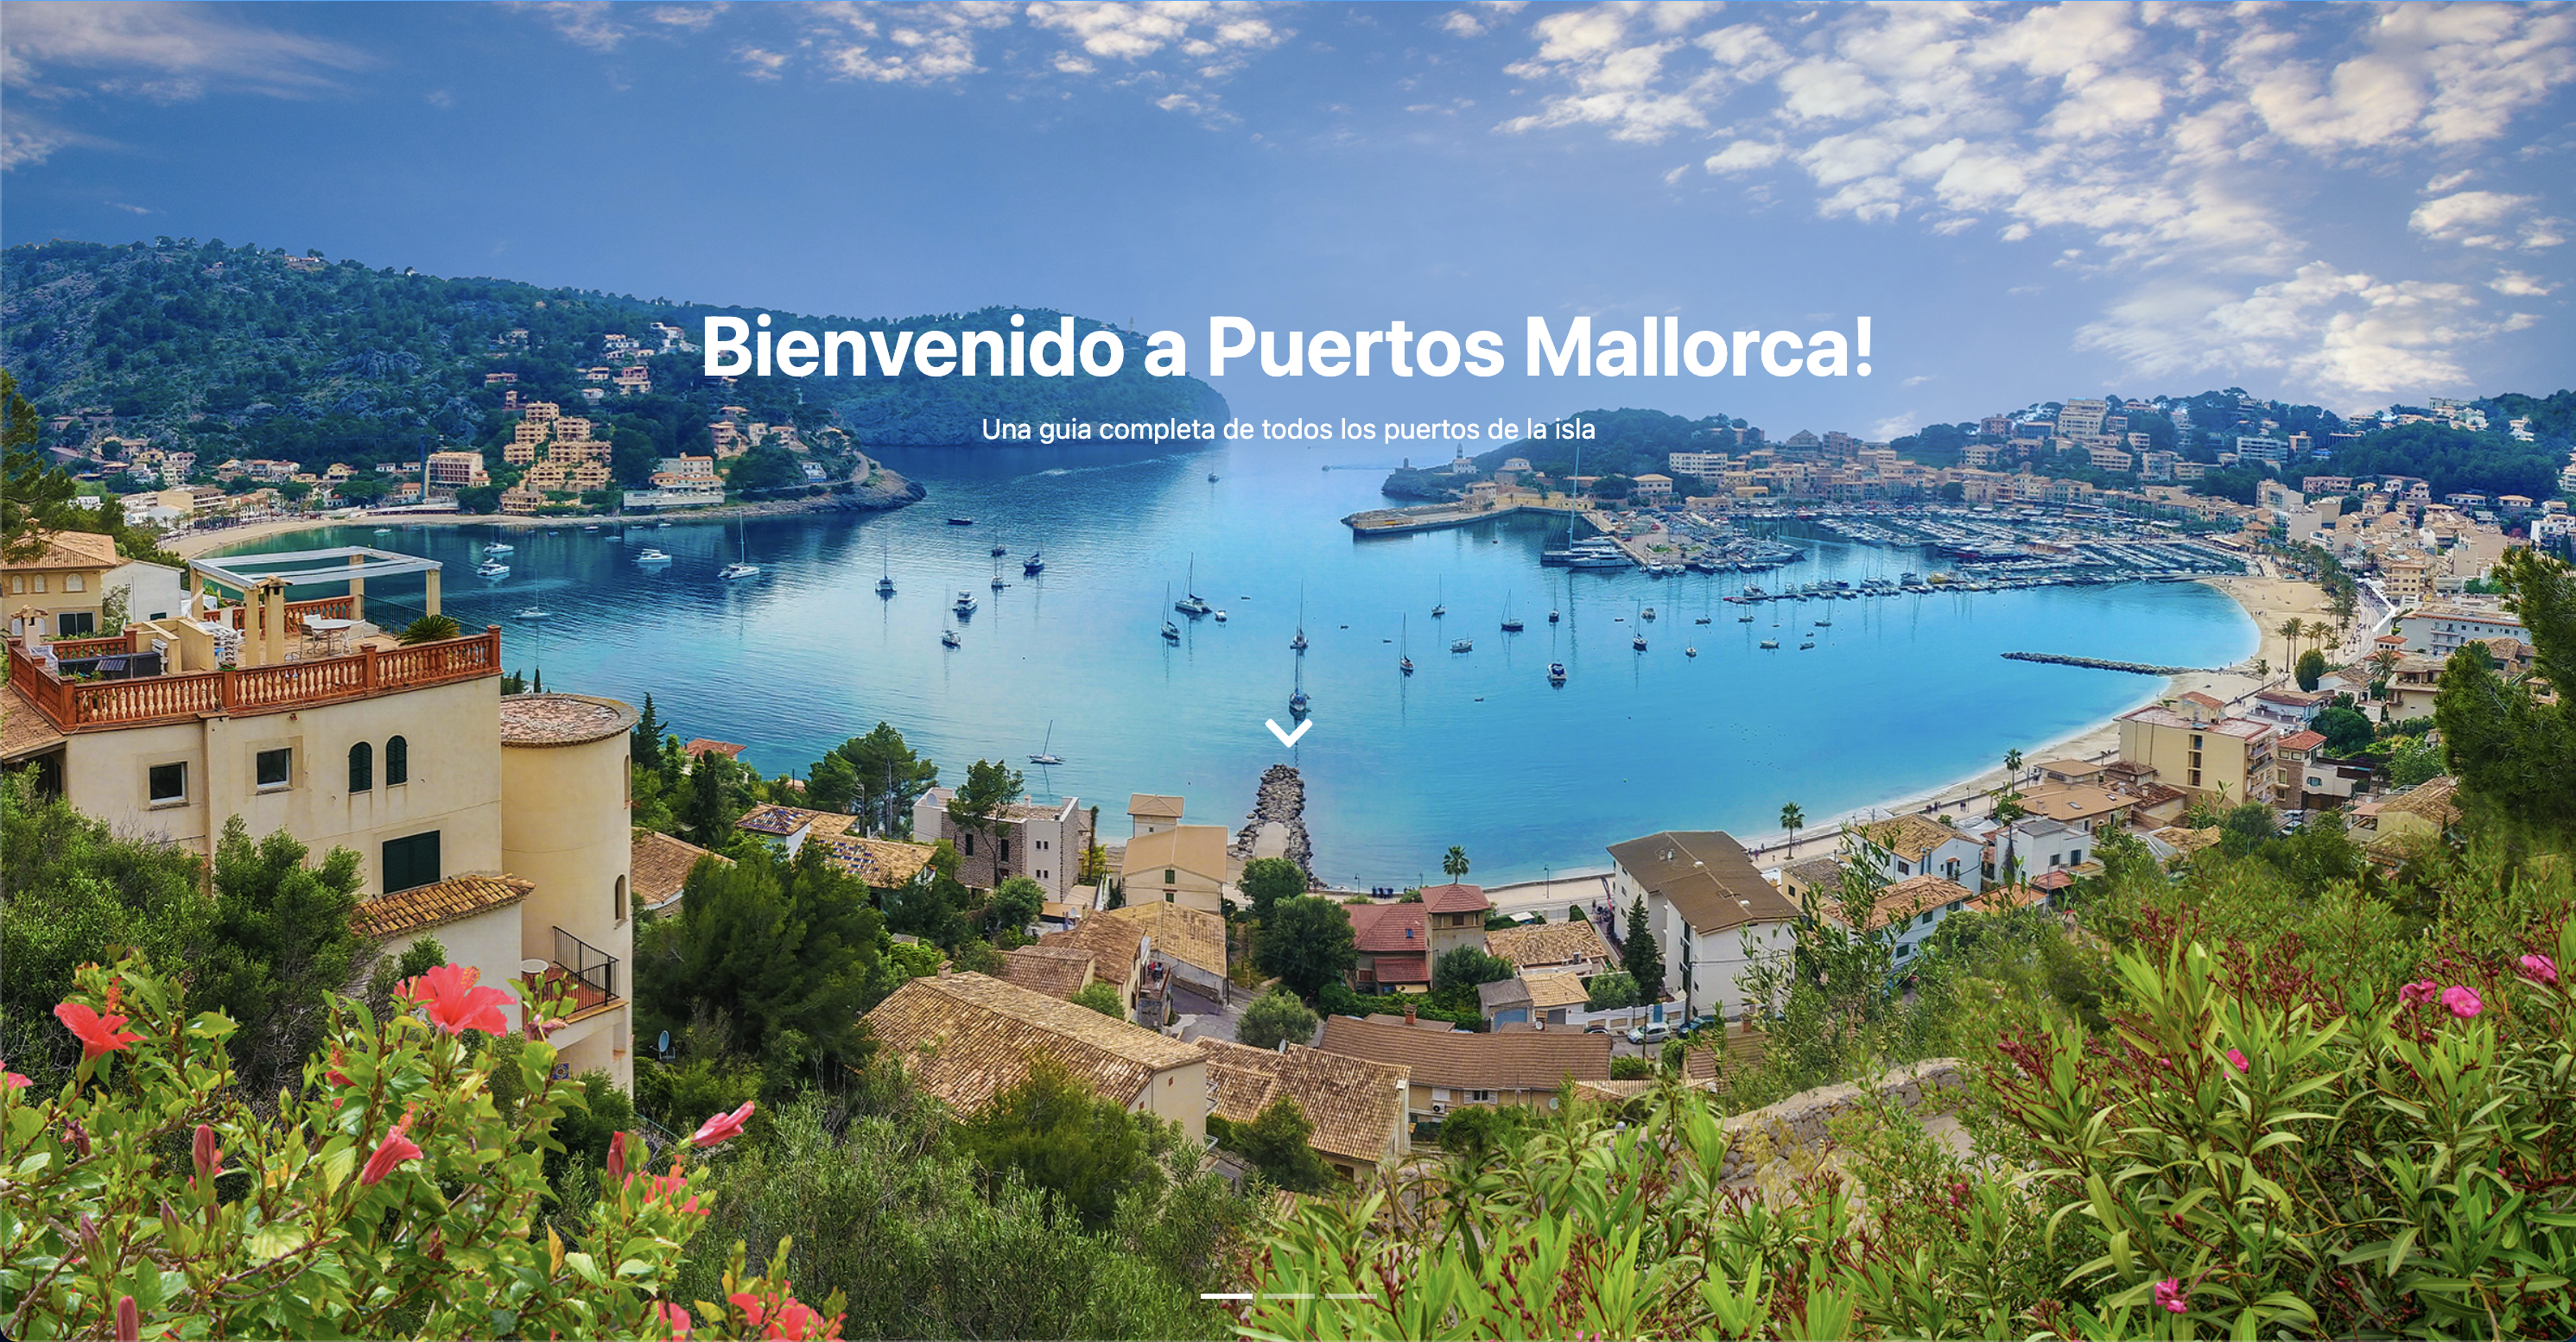
\includegraphics[width=0.4\textwidth]{images/carousel1.png}
    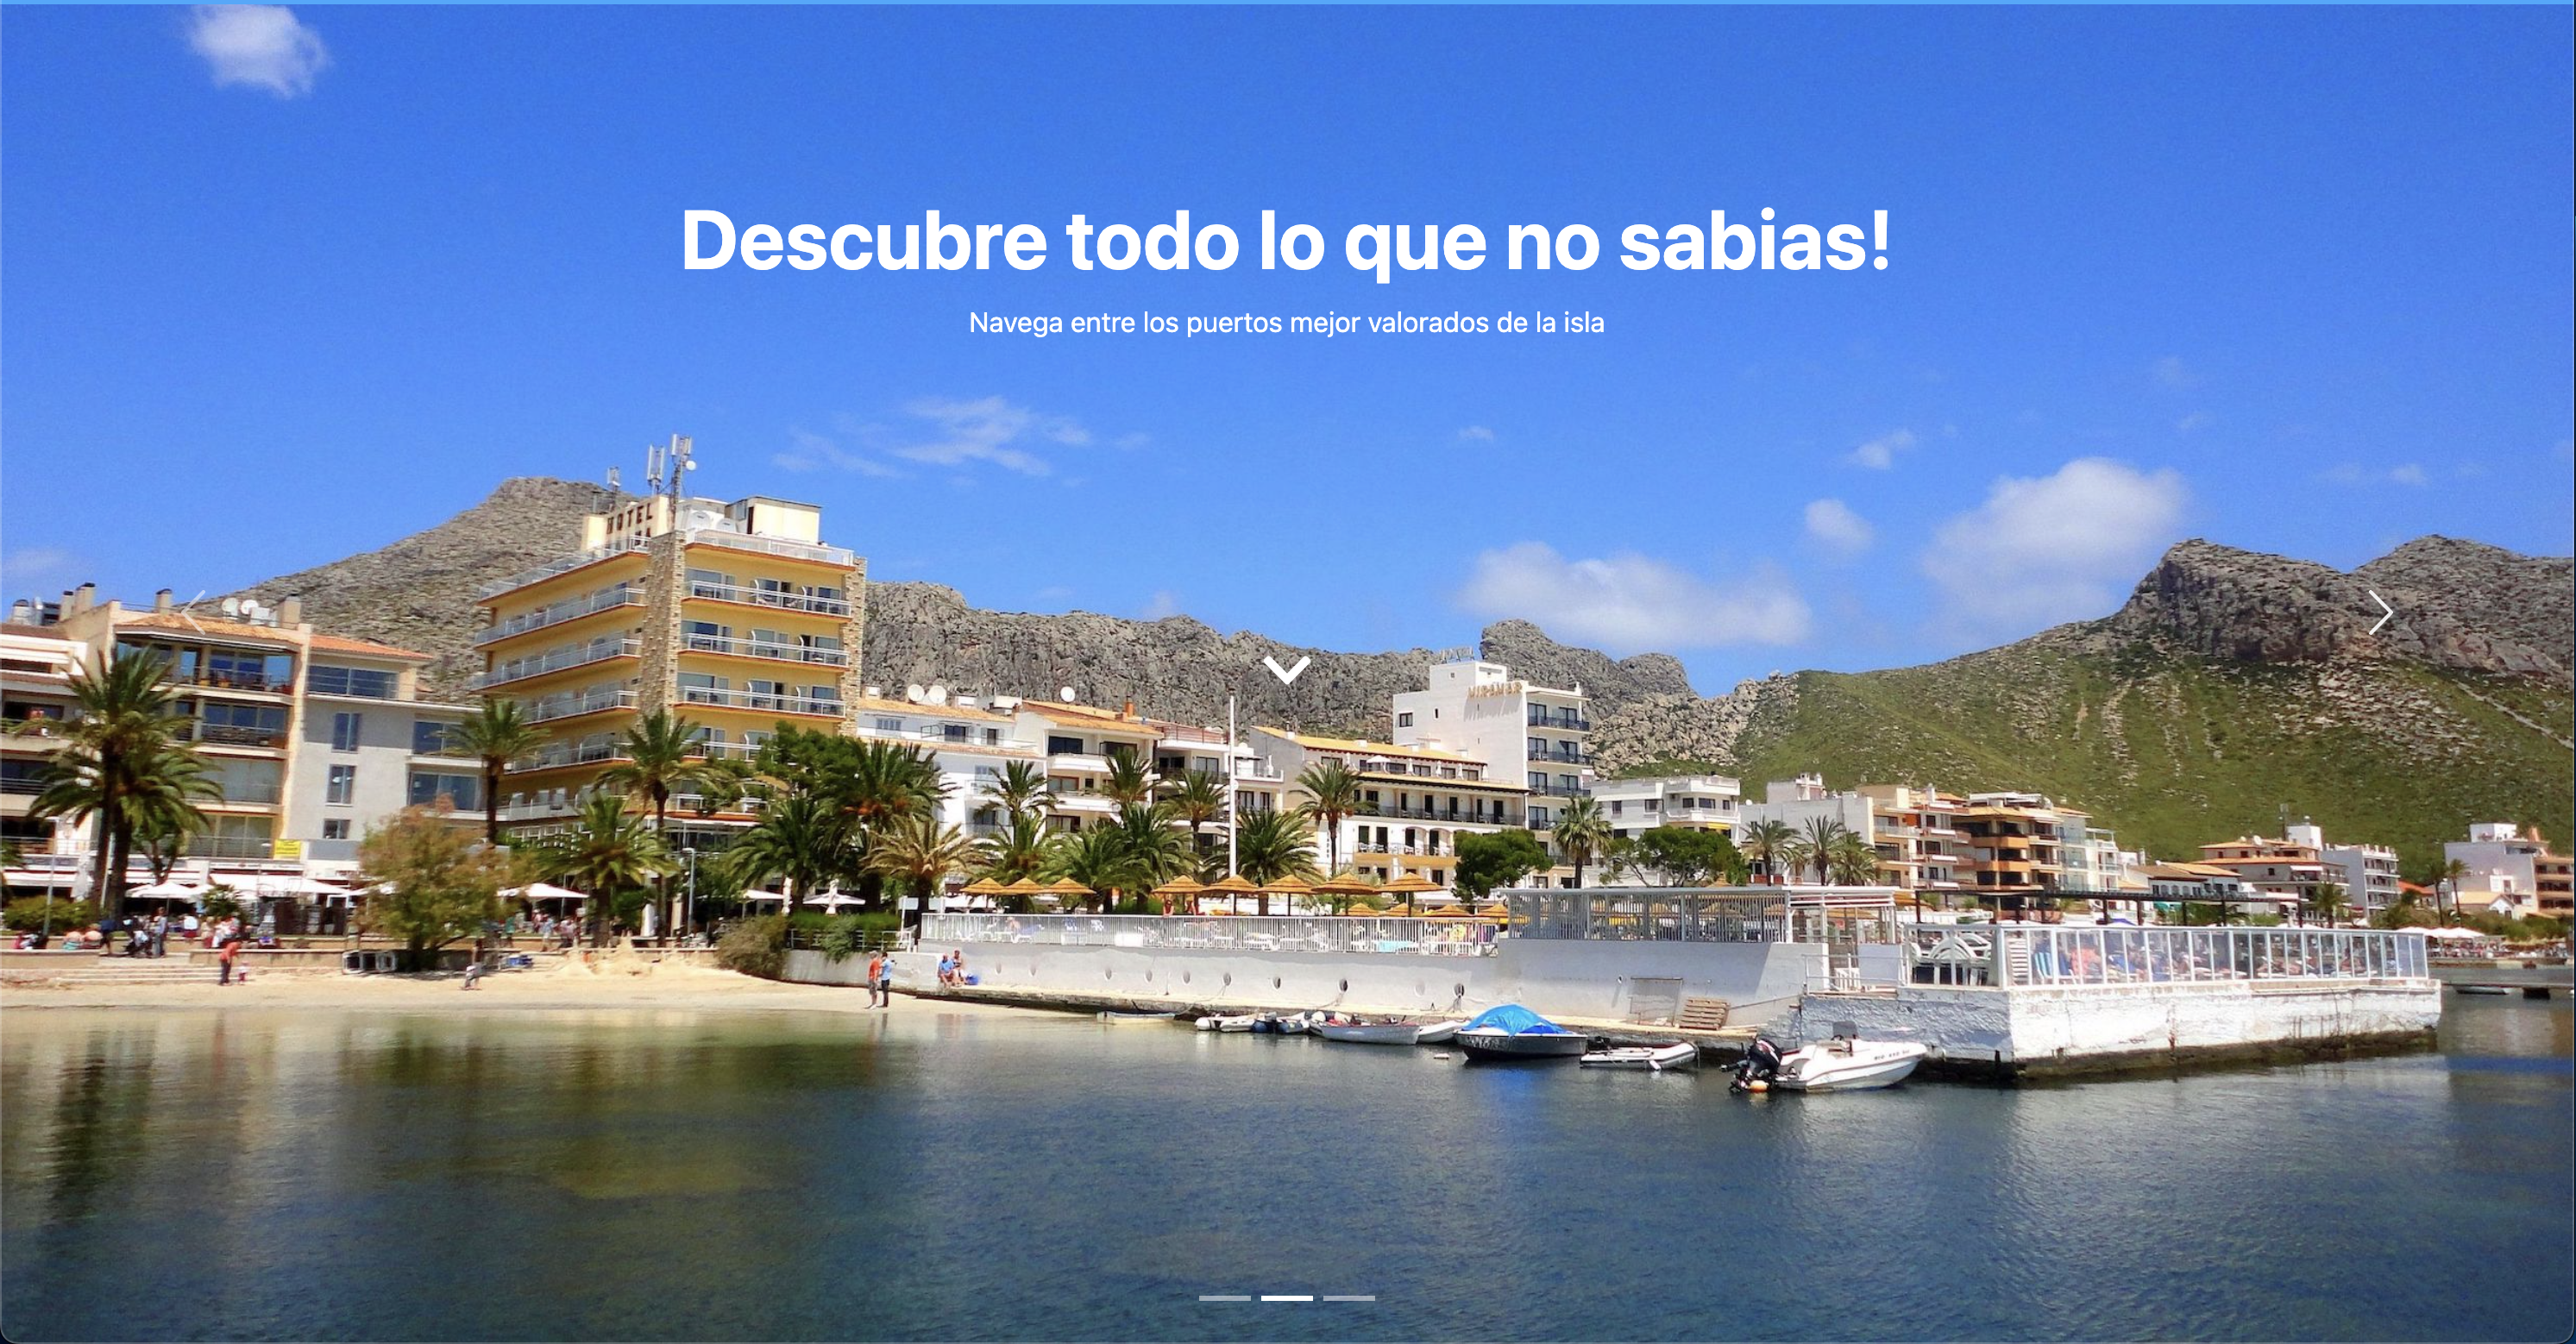
\includegraphics[width=0.4\textwidth]{images/carousel2.png}
    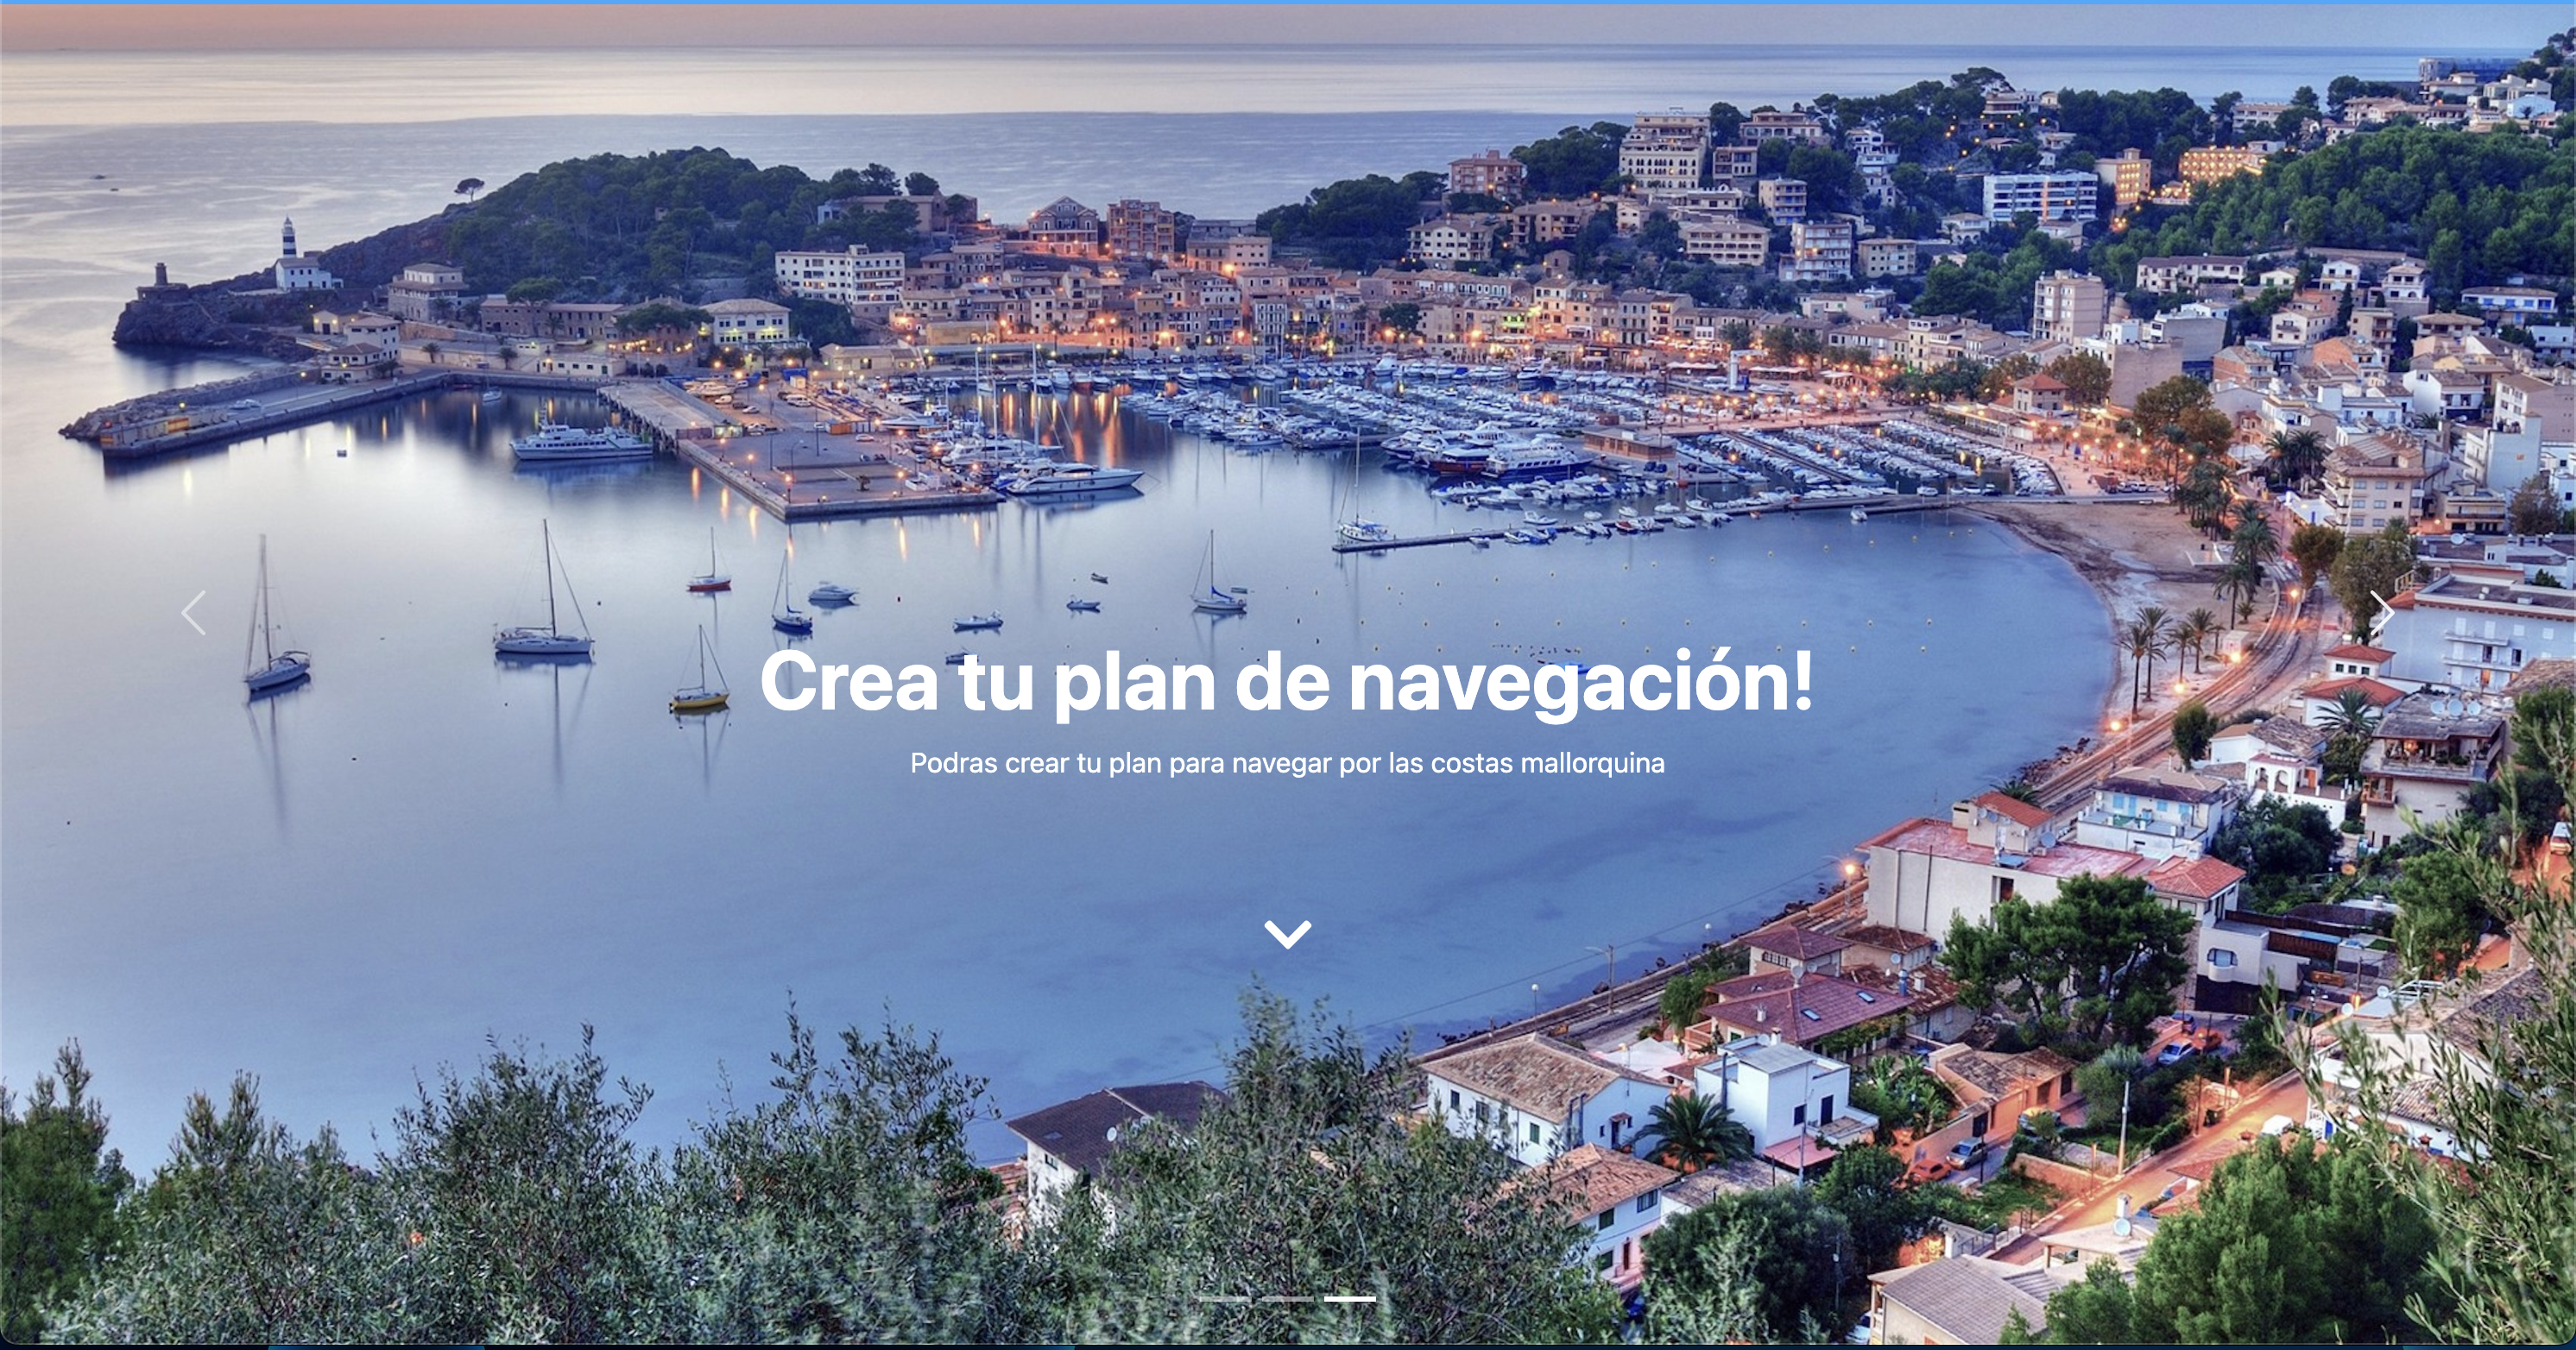
\includegraphics[width=0.4\textwidth]{images/carousel3.png}
    \caption{Las 3 fotos del carousel con sus respectivos textos}
\end{figure}

\noindent Una vez pasamos el carousel de fotos, llegamos a la parte introductoria de la pagina, donde hay una pequeña descripción en forma de texto muy concido sobre lo que se puede hacer en la página.
\begin{figure}[ht]
    \centering
    \includegraphics[width=1.0\textwidth]{images/introduccion.png}
    \caption{Sección introductoria de la web-app}
\end{figure}
\subsection{Pagina de un Puerto}
\subsection{Plan de Navegación}
\subsection{Pagina de Contacto}

\noindent 
\section{Herramientas i Liberrias}
\end{document}